% Preamble
\documentclass[11pt]{article}
% Packages
\usepackage{ngerman}
\usepackage{amsmath}
\usepackage{url}
\usepackage{graphicx}
\usepackage{float}
\usepackage{pifont}
% Title ToC

\title{\textbf{Konzepte} zur Bachelorarbeit\\\large{Template-basierte Synthese von\\Verzweigungsstrukturen mittels
L-Systemen}}
\author{Adrian Helberg}

% Document
\begin{document}
    \maketitle
    \tableofcontents
    \newpage
    \section{Softwareprojekt}
    \subsection{Vorgehensmodell}
    Eine Fallstudie der Universität Karlsruhe\cite{1} untersucht den Einsatz der Softwaretechnik \textbf{Extreme Programming}
    (XP) im Kontext der Erstellung von Abschlussarbeiten im Universitätsumfeld.\\~\\
    Hierzu werden folgende Schlüsselpraktiken untersucht:
    \begin{itemize}
        \item XP als Softwaretechnik zur schrittweisen Annäherung an die Anforderungen eines Systems
        \item Änderung der Anforderungen an das Systems
        \item Funktionalitäten (\textbf{Features}) werden als Tätigkeiten des Benutzers (\textbf{User Stories}) definiert
        \item Zuerst werden Komponententests (Modultests) geschrieben und anschließend die Features (Test-driven Design)
        \item Keine seperaten Testing-Phasen
        \item Keine formalen Reviews oder Inspektionen
        \item Regelmäßige Integration von Änderungen
        \item Gemeinsame Implementierung (Pair Programming) in Zweiergruppen
    \end{itemize}
    Aus der Fallstudie geht hervor, dass Extreme Programming einige Vorteile bei der Bearbeitung eines Softwareprojektes
    einer Bachelorarbeit bietet.
    Zum einen können sich Anforderungen an das zu erstellende System durch parallele Literaturrecherche ändern, zum
    anderen können die Arbeitspakete durch Releases abgedeckt werden.
    \newpage

    \subsection{Vorgehen}
    Das Programm zu dieser Arbeit wird mit einem XP-basierten Ansatz erarbeitet.
    Hierbei beinhaltet ein \textbf{Release} Funktionen, die insgesamt für eine neue Version des Systems ausreichen;
    also ein vollständig funktionsfähiges Programm liefern.
    \textbf{User Stories} sind innerhalb der Iterationen umzusetzende Teilaufgaben und deren Aufwandseinschätzung gibt
    Auskunft über den Entwicklungsaufwand einer Umsetzung.\\~\\
    Umsetzung des Softwareprojektes in Iterationen mit folgenden Phasen:
    \begin{itemize}
        \item Planung:
        \begin{itemize}
            \item Release-Planung:\\"`\textit{Welche Features werden in diesem Release umgesetzt?}"',\\User Stories,
            Aufwandsschätzung, Anforderungsmanagement
            \item Iterationsplanung:\\Umwandlung der User Stories in kleine Arbeitsschritte,\\Festlegen der Dauer einer
            Implementierung
        \end{itemize}
        \item Entwurf: Architektur, Klassendiagramme, Schnittstellen
        \item Testing: (Automatisierte) Modul- und Regressionstests
        \item Programmierung: Umsetzung der Features, Implementierung, Modularisierung
    \end{itemize}
    \begin{figure}[H]
        \centering
        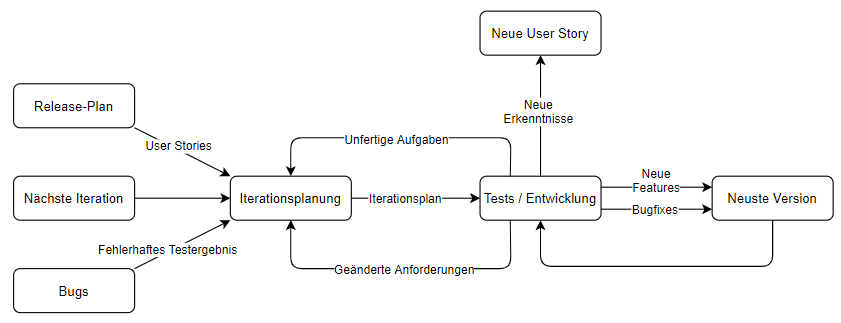
\includegraphics[width=15cm]{../images/extreme_programming.PNG}
        \caption{Ablaufdiagramm}
    \end{figure}

    \subsection{Technnologien}
    \begin{itemize}
        \item Programmiersprache: Java Version X mit
        \begin{itemize}
            \item JavaFX Version X
        \end{itemize}
        \item Build-Management-Tool: Gradle\cite{gradle} Version X
        \item Versionskontrolle: Github Repository\cite{github} via Git\cite{git}
        \item IDE: JetBrains IntelliJ IDEA\cite{idea} 2020.2.2 (Ultimate Edition)
        \item Betriebssystem: Microsoft Windows 10 Pro 64 Bit
        \item Prozessor: Intel Core i5-3570K CPU @ 3.40GHz
        \item User Story Map: Trello Board\cite{trello}
    \end{itemize}

    \newpage

    \section{Dokumentation}
    \subsection{Gliederung}
    Im Folgenden wird eine vorläufige Gliederung der schriftlichen Ausarbeitung gezeigt
    \begin{itemize}
        \item[1.] Abbildungs- und Tabellenverzeichnis
        \item[2.] Abkürzungsverzeichnis
        \item[3.] Einleitung
        \begin{itemize}
            \item[3.1.] Problemstellung
            \item[3.2.] Ziele
            \item[3.3.] Methodik
            \item[3.4.] Aufbau
        \end{itemize}
        \item[4.] Grundlagen
        \begin{itemize}
            \item[4.1.] Grundbegriffe
            \item[4.2.] Grundlegende Arbeiten
            \item[4.3.] Verwandte Arbeiten
        \end{itemize}
        \item[5.] Konzepte
        \begin{itemize}
            \item[5.1.] Probleme \& Lösungsansätze
            \item[5.2.] Architektur
            \item[5.3.] Algorithmen
        \end{itemize}
        \item[6.] Implementierung
        \item[7.] Evaluierung
        \begin{itemize}
            \item[7.1.] Testumgebung
            \item[7.2.] Beobachtungen \& Ergebnisse
            \item[7.3.] Diskussion und Bewertung
        \end{itemize}
        \item[8.] Ausblick
        \item[9.] Literaturverzeichnis
        \item[10.] Eidesstattliche Erklärung
    \end{itemize}

    \section{Releases}
    Dieses Kapitel beschreibt die Release-Planung des Softwareprojekts im Sinne eines XP-orientierten Ansatzes:\\
    Zuerst werden die Funktionalitäten, die im entsprechenden Release umgesetzt werden sollen definiert und \textbf{Epics}
    zugeteilt.
    Anschließend werden feingranulare User Stories formuliert, die mit einer Aufwandseinschätzung versehen werden.
    Parallel findet das Anforderungsmanagement (\textit{engl. Requirements Engineering}), das sich mit der Steuerung,
    Kontrolle und Verwaltung der Anforderungen an das System beschäftigt, statt.
    Mit diesen Informationen lässt sich dann die Iterationsplanung umsetzen.
    Die Umwandlung der User Stories in Arbeitsschritte (\textbf{Tasks}) und das Festlegen deren Dauer wird hier umgesetzt.

    \subsection{Release 1}
    Erstellung einer grafischen Benutzeroberfläche zur Erstellung von Verzweigungsstrukturen\\
    \textit{Siehe Exposé Kapitel 1.1.2 Überblick Punkt I. Strukturieren und II. Visualisieren}\\~\\
    \begin{figure}[H]
        \centering
        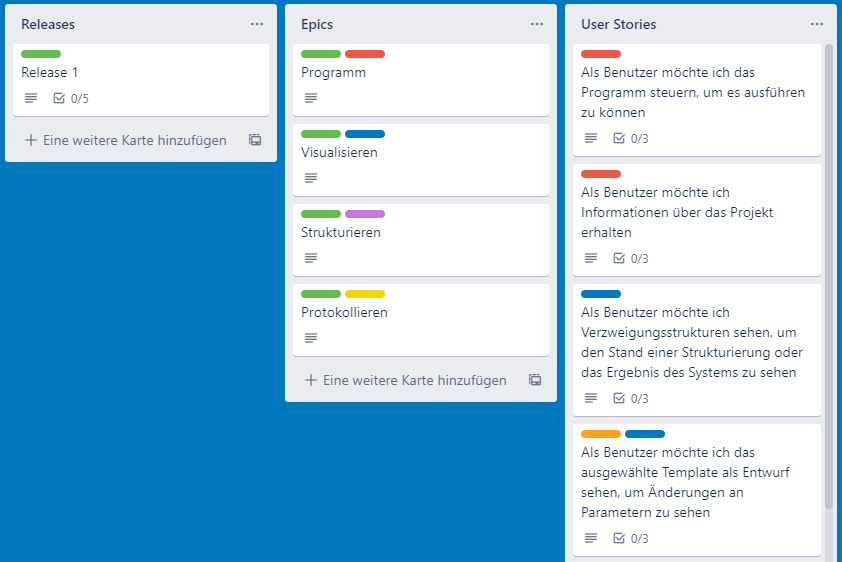
\includegraphics[width=12cm]{../images/User_Story_Map.PNG}
        \caption{User Story Map mit Releases, Epics und User Stories}
    \end{figure}

    \subsection{Release 2}

    \section{Implementation}
    Da die Arbeitspakete (Releases) iterativ und abgeschlossen erarbeitet werden, wird das
    \textbf{Pipeline} Design Pattern\cite{pipeline} genutzt.

    \newpage

    ~\nocite{*}
    \renewcommand{\refname}{Quellen}
    \bibliography{konzepte}
    \bibliographystyle{plain}
    \addcontentsline{toc}{section}{Quellen}

\end{document}